\chapter{Unstable Gradients}

\begin{exercise}
Can we avoid the vanishing gradient problem by using a different activation function 
than the sigmoid function?
\end{exercise}
\begin{solution}
If we use an activation function~$f$ whose derivative is higher at $f'(0)$ is higher, but
less than $1$, we can reduce the severity of the vanishing gradient problem, but not eliminate 
it altogether. If we were choose $f$ such that $f'(0) > 1$, then we might end up with the 
exploding gradient problem. 

One such candidiate function is the hyperbolic tangent function. This is defined as:
\[
    \tanh (x) = \frac{e^x - e^{-x}}{e^x + e^{-x}}.
\]
The derivative of this function is $\tanh ' (x) = 1 - \tanh (x)^2$. The graph of the 
function and its derivative is shown in Figure~\ref{fig:tanh}.

\begin{figure}[ht]
\begin{center}
\begin{minipage}[b]{0.4\textwidth}
\begin{center}
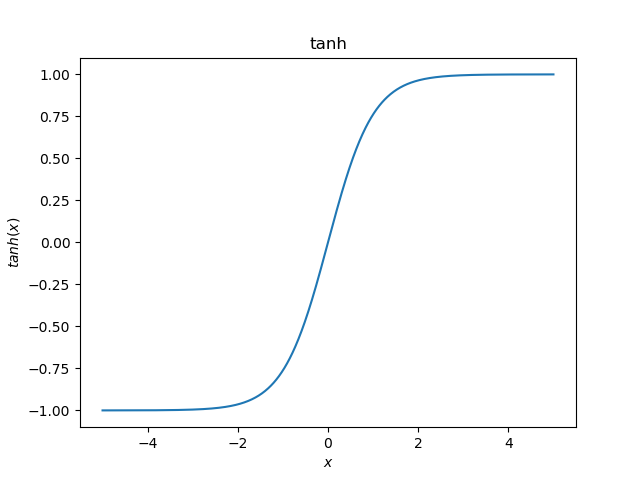
\includegraphics[width=\textwidth]{Tanh.png}
\end{center}
\end{minipage}
\begin{minipage}[b]{0.4\textwidth}
\begin{center}
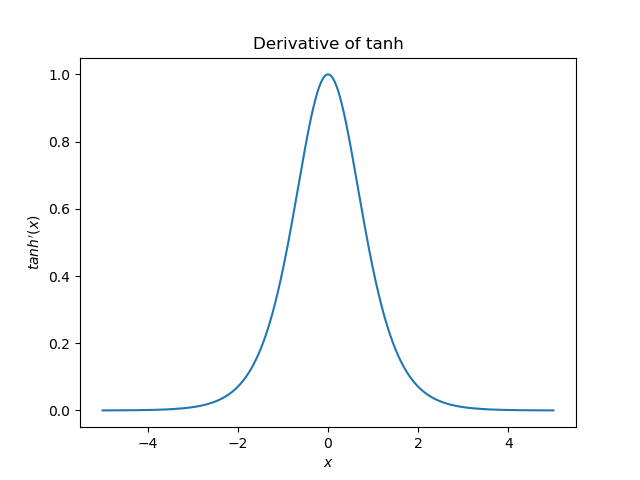
\includegraphics[width=\textwidth]{TanhDerivative.png}
\end{center}
\end{minipage}
\caption{The Tanh function and its derivative}
\label{fig:tanh}
\end{center}
\end{figure}
\end{solution}
